\documentclass{article}
\usepackage{tikz}
\usepackage{amsmath, amssymb}
\usetikzlibrary{calc, positioning, backgrounds, fit}

\begin{document}
	
	\begin{figure}[htbp]
		\centering
		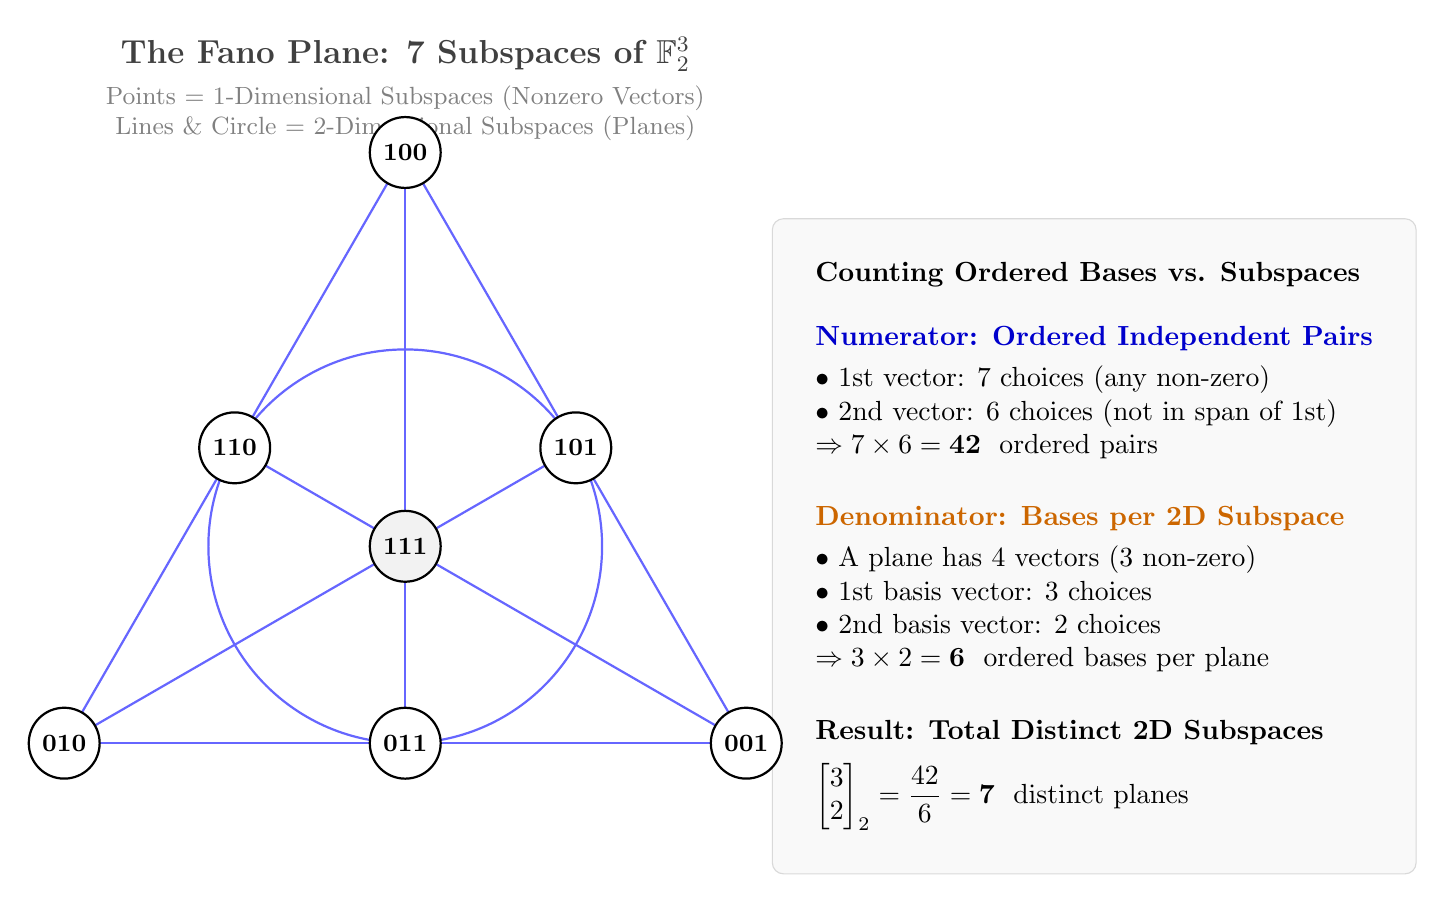
\begin{tikzpicture}[
			scale=2.5,
			font=\sffamily,
			% Node styles
			vecNode/.style={circle, fill=white, draw=black, thick, inner sep=2pt, minimum size=9mm, font=\small\bfseries},
			% Line styles
			subspaceLine/.style={thick, draw=blue!60},
			textPanel/.style={align=left, font=\normalsize}
			]
			
			% =========================================================
			% 1. THE FANO PLANE (Incidence Geometry of F_2^3)
			% =========================================================
			
			\begin{scope}[shift={(0,0)}]
				% Title
				\node[font=\large\bfseries, align=center, text=darkgray] at (0, 2.5) {The Fano Plane: 7 Subspaces of $\mathbb{F}_2^3$};
				\node[font=\small, align=center, text=gray] at (0, 2.2) {Points = 1-Dimensional Subspaces (Nonzero Vectors)\\Lines \& Circle = 2-Dimensional Subspaces (Planes)};
				
				% Define Coordinates for Fano Plane (Equilateral Triangle)
				\coordinate (V100) at (90:2);
				\coordinate (V010) at (210:2);
				\coordinate (V001) at (330:2);
				
				\coordinate (V110) at ($(V100)!0.5!(V010)$);
				\coordinate (V011) at ($(V010)!0.5!(V001)$);
				\coordinate (V101) at ($(V100)!0.5!(V001)$);
				
				\coordinate (V111) at (0,0); % Center
				
				% Draw Subspace Lines (The 7 Planes)
				% 1-3: Outer edges
				\draw[subspaceLine] (V100) -- (V010);
				\draw[subspaceLine] (V010) -- (V001);
				\draw[subspaceLine] (V001) -- (V100);
				
				% 4-6: Altitudes (Medians going through the center)
				\draw[subspaceLine] (V100) -- (V011);
				\draw[subspaceLine] (V010) -- (V101);
				\draw[subspaceLine] (V001) -- (V110);
				
				% 7: The "Circle" Line (The 7th Subspace)
				\draw[subspaceLine] (V111) circle (1);
				
				% Draw Nodes (The 7 Nonzero Vectors)
				\node[vecNode] at (V100) {100};
				\node[vecNode] at (V010) {010};
				\node[vecNode] at (V001) {001};
				
				\node[vecNode] at (V110) {110};
				\node[vecNode] at (V011) {011};
				\node[vecNode] at (V101) {101};
				
				\node[vecNode, fill=gray!10] at (V111) {111};
			\end{scope}
			
			% =========================================================
			% 2. THE COUNTING BREAKDOWN (Right Panel)
			% =========================================================
			
			\begin{scope}[shift={(3.5, 0)}]
				\node[textPanel] (mathPanel) at (0,0) {
					\textbf{Counting Ordered Bases vs. Subspaces}\\[4mm]
					\text{\textcolor{blue!80!black}{\textbf{Numerator: Ordered Independent Pairs}}}\\[1mm]
					$\bullet$ 1st vector: 7 choices (any non-zero)\\
					$\bullet$ 2nd vector: 6 choices (not in span of 1st)\\
					$\Rightarrow 7 \times 6 = \mathbf{42}$ \text{ ordered pairs}\\[5mm]
					
					\text{\textcolor{orange!80!black}{\textbf{Denominator: Bases per 2D Subspace}}}\\[1mm]
					$\bullet$ A plane has 4 vectors (3 non-zero)\\
					$\bullet$ 1st basis vector: 3 choices\\
					$\bullet$ 2nd basis vector: 2 choices\\
					$\Rightarrow 3 \times 2 = \mathbf{6}$ \text{ ordered bases per plane}\\[5mm]
					
					\text{\textbf{Result: Total Distinct 2D Subspaces}}\\[2mm]
					$\displaystyle \begin{bmatrix} 3 \\ 2 \end{bmatrix}_2 = \frac{42}{6} = \mathbf{7}$ \text{ distinct planes}
				};
				
				% Background box for math panel
				\begin{scope}[on background layer]
					\node[fill=gray!5, draw=gray!30, rounded corners, fit=(mathPanel), inner sep=12pt] {};
				\end{scope}
			\end{scope}
			
		\end{tikzpicture}
	\end{figure}
	
\end{document}